\documentclass{beamer}
\usepackage{graphicx}
\usepackage[english]{babel}
\usepackage{hyperref}
\usepackage{multicol}
\usepackage{amssymb}
\usepackage{amsmath}
\usepackage{graphicx}


\usepackage{xcolor}
\usepackage{tikz}
\usetikzlibrary{calc}

\mode<presentation>
{ 
	\usetheme{Berkeley}
    \usecolortheme{default}
    \usefonttheme{structurebold}
}


\title[University of Michigan LoG(M)]{Hilbert Polynomials and Monomial Ideals}
\author{Joe Donato \and Zijian Zhang \and Faustas Udrenas }
\institute{University of Michigan}
\date{Last update \today}


\begin{document}
\begin{frame}
\titlepage
\end{frame}


% ZIJIAN SLIDES INTRODUCTION 

% JOE SLIDES HISTORICAL CONTEXT/MOTIVATION

\begin{frame}
	\frametitle{Our Progress}
	\begin{enumerate}
	\item We have been able to count the number of saturated ideals for all hilbert polynomials in two and three variables (N=1 and N=2 respectively)
	\item We have constructed a brute force algorithm that will determine a $\lambda$ partition for any $n^{th}$ degree Hilbert polynomial
	\end{enumerate}
\end{frame}

\begin{frame}
	\frametitle{Macaulays Theorem}
	\begin{theorem}
   Let $p(d)$ be a polynomial in one variable. $p(d)$ is a Hilbert Polynomial if and only if $p(d)$ can be written in the form 
   \[\sum_{i=1}^{r}\binom{d+\lambda_i -i}{\lambda_i -1}\] for some $\lambda= (\lambda_1,\hdots,\lambda_r)$  where $N \geq \lambda_1 \geq \hdots \geq \lambda_r \geq 1$. Where N is the number of variables minus one.

	\end{theorem}
	We can use this theorem to help us count the number of saturated ideals:
\end{frame}


\begin{frame}
	\frametitle{Our approach}
	Given a Hilbert Polynomial and Number of Variables N+1
	\begin{enumerate}
	\item Find the $\lambda$ - partition of $H_I(d)$ 
	\item Use the $\lambda_i$'s to count, combinatorially, the number of saturated ideals in N+1 variables
	\end{enumerate}
\end{frame}

\begin{frame}
	\frametitle{Counts in 2 Variables (N=1)}
	\begin{itemize}
	\item Any Hilbert Polynomial $H_I(d)$ for $N=1$ must be a constant polynomial
	\item By Macaulys Theorem, the $\lambda_i$ values in our $\lambda$- partion can be at most 1.
	\begin{itemize}
		\item Thus \[ \binom{d+\lambda_i -i}{\lambda_i-1} = \binom{d+1-i}{0} =1
		\]
	\end{itemize}
	\end{itemize}
\end{frame}

\begin{frame}
	\frametitle{Counts in 2 Variables (N=1)}
	\begin{itemize}
	\item Example: $H_I(d)=3 \;\; \implies \lambda = (1,1,1) $ \;\; 3 "rows".
	\item So how many of these saturated ideals can we have?
	\begin{itemize}
		\item We can answer this by asking "how many ways can we place 3 'rows' in two 'directions' (x or y)"
		\item The problem has now been effecitvely reduced to a simple counting problem (A weak composition of 3 objects into 2 boxes).
	\end{itemize}
	\item In this case, it turns out to be 4 

	\end{itemize}
\end{frame}


\begin{frame}
	\frametitle{First Orientation}
	\begin{center}
	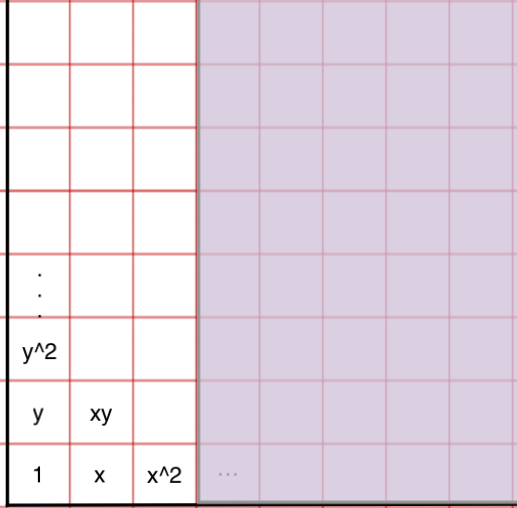
\includegraphics[width=6cm, height=6cm]{LogMMidtermPresentationImages/hpis3firstorientation.png}
	\end{center}
\end{frame}

\begin{frame}
	\frametitle{Second Orientation}
	\begin{center}
		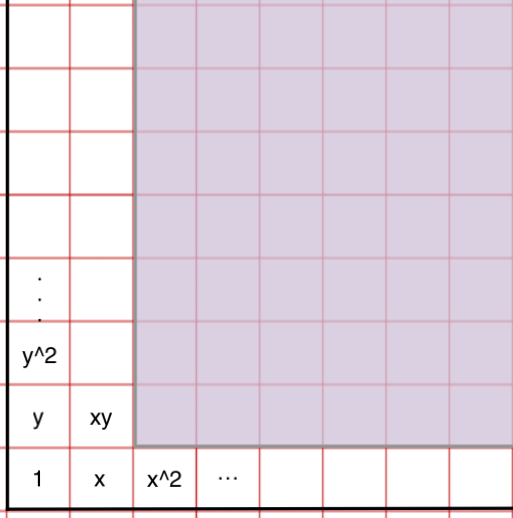
\includegraphics[width=6cm, height=6cm]{LogMMidtermPresentationImages/hpis3secondorientation.png}
	\end{center}
\end{frame}

\begin{frame}
	\frametitle{Third Orientation}
	\begin{center}
	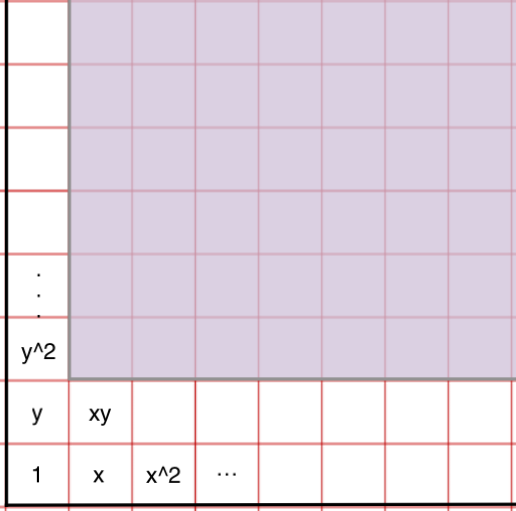
\includegraphics[width=6cm, height=6cm]{LogMMidtermPresentationImages/hpis3thirdorientation.png}
	\end{center}
\end{frame}


\begin{frame}
	\frametitle{Fourth Orientation}
	\begin{center}
	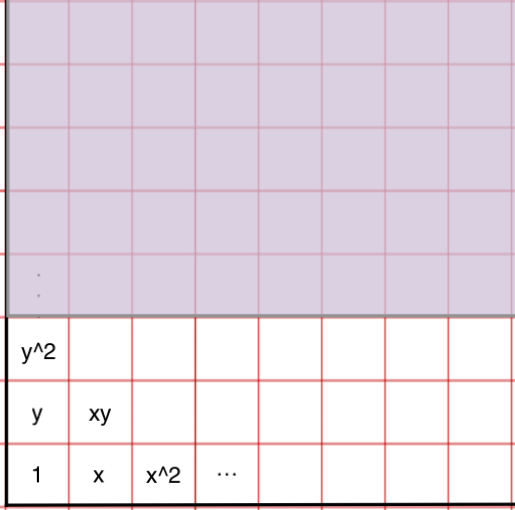
\includegraphics[width=6cm, height=6cm]{LogMMidtermPresentationImages/hpis3fourthorientation.png}
	\end{center}
\end{frame}

\begin{frame}
	\frametitle{Generalizing the counts for two dimensions}
	\begin{itemize}
	\item If $H_I(d)= k$ for some positive constant k then $\lambda = {(1^{[k]})}$
	\item This means we have k "rows" to place in two directions
	\item Thus, how many ways can we place k objects into 2 boxes?
	\item This is a weak composition
	\[\binom{k+2-1}{2-1}= \binom{k+1}{1} = k+1\]
	\item We conclude that for any positive constant polynomial $p(d)$  there are $k+1$ ideals I, up to saturation, such that $H_I(d)= p(d)$ in two variables{}
	\end{itemize}
\end{frame}

\begin{frame}
	\frametitle{Counts in 3 Variables (N=2)}
	So what about 3 variables?
	\begin{itemize}
	\item Similar approach, but slightly more complex
	\begin{enumerate}
	\item Now our Hilbert Polynomials $H_I(d)$ can be linear in d
	\item This implies $\lambda$-partition can have lambda values of 2 and 1
	\end{enumerate}
	\item A lambda value of 2 corresponds to placeing 2d-planes in the xyz-grid
	\item so now we have to count the number of ways to place a combination of planes and rows in 3-space.
	\end{itemize}
\end{frame}

\begin{frame}
	\frametitle{Counts in 3 Variables (N=2)}
	Our approach is...
	\begin{enumerate}
	\item Find $\lambda$. 
	\begin{itemize}
		\item The number of '2's in $\lambda$ tells us how many planes we must place
		\item The number of '1's in $\lambda$ tells us how many rows we must place
	\end{itemize}
	\item Count the number of ways to place planes first
	\item Count the number of ways to place rows second
	\item Product of these two values together give us the final count final count
	\end{enumerate}
\end{frame}

\begin{frame}
	\frametitle{Counts in 3 Variables (N=2)}
	\begin{itemize}
	\item The advantage of placing our planes first is that when we do so, we are not changing the "form" of the space we are working with.
	\item Thus, if we count the number of ways to place a given number of planes, we are still left with something that resembles 3-space
	\end{itemize}
\end{frame}

\begin{frame}
	\frametitle{Example}
	\begin{itemize}
	\item Consider the Hilbert Polynomial $H_I(d) = 2d+3$
	\item Here $\lambda = (2,2,1,1)$
	\item So we have 2 planes to place in 3-space
	\end{itemize}
\end{frame}


\begin{frame}
	\frametitle{Example Continued}
	\begin{center}
	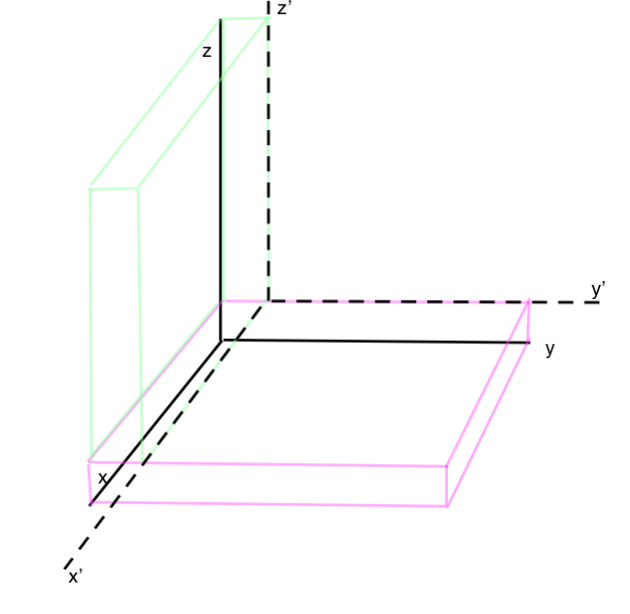
\includegraphics[width = 6cm, height = 6cm]{LogMMidtermPresentationImages/shifting3spacegood.png}
	\end{center}
\end{frame}


\begin{frame}
	\frametitle{Example Continued}
	\begin{itemize}
	\item From here, the question is reduced down to finding the number of ways to place a given number of rows in 3-space
	\item So, how many ways can we place two rows in 3 different directions?
	\item Again this is a weak composition of 2 objects into 3 rows
	\item HOWEVER, in each composition, we must consider the number of ways to orient two rows if they happen to be facing in the same direction 
	\end{itemize}
\end{frame}



\begin{frame}
	\frametitle{First Orientation of Two Rows in the X-direction}
	\begin{center}
	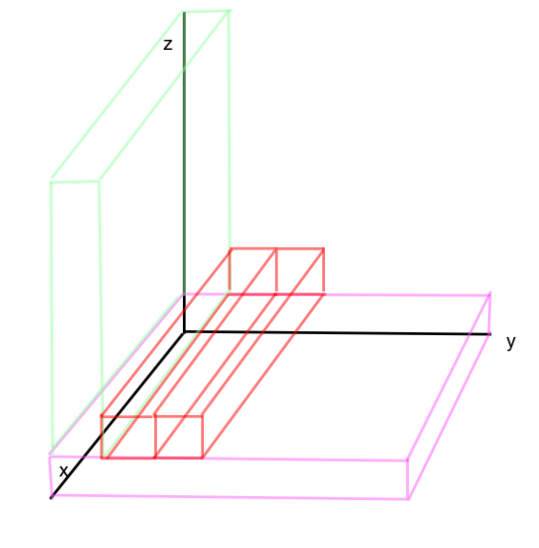
\includegraphics[width = 6cm, height = 6cm]{LogMMidtermPresentationImages/2rowsfirstorientation3space.png}
	\end{center}
\end{frame}

\begin{frame}
	\frametitle{Second Orientation of Two Rows in the X-direction}
	\begin{center}
	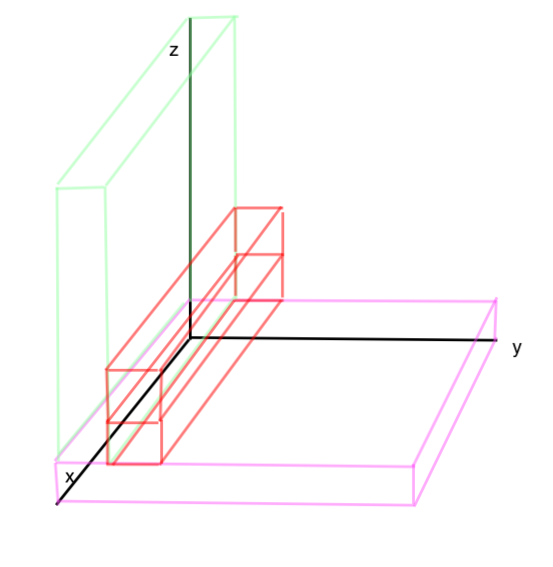
\includegraphics[width = 6cm, height = 6cm]{LogMMidtermPresentationImages/2rowssecondorientation3space.png}
	\end{center}
\end{frame}

\begin{frame}
	\frametitle{The Generalized count for N=2}
	Given $H_I(d)$, then $\lambda_{H_I} = (2^{p}, 1^{r})$ for some $p,r \geq 0$\\
	The number of saturated ideals is thus given by...
	\[\binom{p+2}{2}\cdot \sum_{i=1}^{\binom{r+2}{2}}\Big[f(c_{x_i})\cdot f(c_{y_i})\cdot f(c_{z_i})\Big]
	\]
	Where $(c_{x_i},c_{y_i}, c_{z_i})$ is the i'th weak composition of r into 3 and f(c) is the number of integer partitions of c
\end{frame}

\begin{frame}
	\frametitle{A Major Obstacle}
	\begin{itemize}
	\item How can we determine $\lambda$? 
	\item Luckily, we have classifications for all linear and quadratic polynomials...
	\end{itemize}
\end{frame}


\begin{frame}
	\frametitle{Some Classifications We Found}
	\begin{enumerate}
				\item Constant
				\[H_I=k \]
				$\lambda$ exists if $K\geq 1$
				\[\lambda = (1^{[k]})\]
				\item Linear
				\[H_I=kd-r\]
				$\lambda$ exists if $r\leq \frac{(k-2)(k-1)}{2}-1$
				\[\lambda = (2^{[k]}, 1^{[\frac{(k-2)(k-1)}{2}-r+1]})\]

	\end{enumerate}
\end{frame}

\begin{frame}
	\frametitle{Some Classifications Continued}
	\begin{enumerate}
				\item Quadratic
				\[H_I=ad^2+bd+c\]
				$\lambda$ exists if
				\begin{enumerate}
					 \item $b > (2a[2-a])$
					\item $c - \frac{1}{3}\big(4a^3-12a^2+11a\big)\geq  \Big[(2a^2-4a-b)(2-2a)-\Big(\frac{(2a^2-4a-b)(2a^2-4a-b+1)}{2}\Big)\Big]$
				\end{enumerate}
	\end{enumerate}
\end{frame}

\begin{frame}
	\frametitle{What about polynomials of degree larger than 2?}
	In order to tackle our main question above, we need to first find our lambda partition. How can we do this for more difficult polynomials? 
\end{frame}

% HERE JOE PUTS IN HIS SLIDES ON THE CODE

\begin{frame}
	\frametitle{Whats Next?}
	\begin{itemize}
	\item Finding the generalized count for Hilbert Polynomials in 4 Variables.
	\item Using discrete differentials to work around the upper bound issue we have in our brute force algorithm. 
	\end{itemize}
\end{frame}

\end{document}



